\documentclass[border=2pt]{standalone}
\usepackage[T1]{fontenc}\usepackage{mathptmx}
\usepackage{amsmath,amssymb}\usepackage{tikz}\usepackage{pgfplots}
\pgfplotsset{compat=1.18}
\usetikzlibrary{shapes.geometric, arrows.meta, positioning, calc}
\setlength{\columnwidth}{3.45in}
\newcommand{\Pfree}{P_{\mathrm{free}}}\newcommand{\dfree}{d_{\mathrm{free}}}\newcommand{\pos}{\mathrm{pos}}
\newcommand{\ind}{\mathbf{1}}\newcommand{\Lin}{\mathcal{L}}
\pgfplotsset{ieeeplot/.style={width=\columnwidth, height=5.4cm,
 tick label style={font=\footnotesize}, label style={font=\footnotesize},
 legend style={font=\footnotesize, draw=black!60, fill=white, fill opacity=0.9, text opacity=1},
 grid=both, grid style={line width=0.2pt, draw=black!15}, major grid style={line width=0.3pt, draw=black!25},
 every axis plot/.append style={line width=0.8pt, mark size=2.2pt}}}
\begin{document}
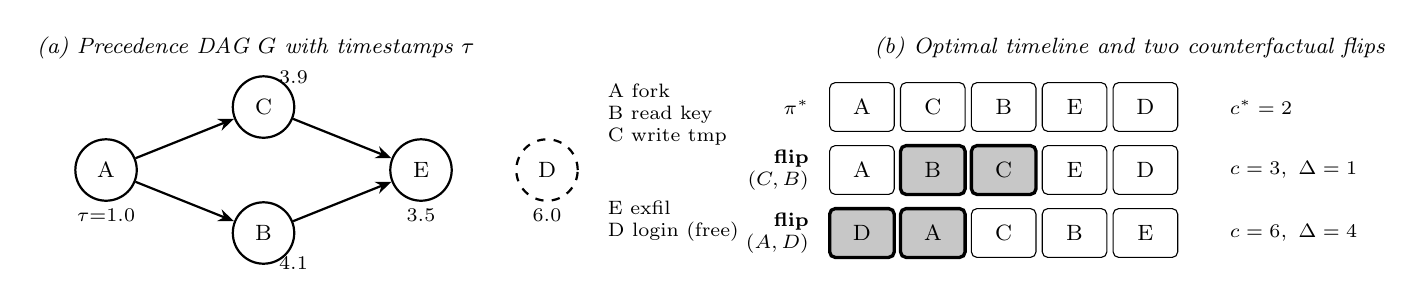
\begin{tikzpicture}[font=\footnotesize,
  ev/.style={circle, draw=black, thick, minimum size=0.78cm, inner sep=0pt, fill=white},
  evf/.style={ev, dashed},
  dag/.style={-{Stealth[length=2mm,width=1.6mm]}, thick},
  cell/.style={draw=black, rounded corners=2pt, minimum width=0.82cm, minimum height=0.62cm, inner sep=1pt},
  swp/.style={cell, fill=black!22, very thick},
  lab/.style={font=\footnotesize\itshape}]
% (a) DAG
\node[lab] at (1.9,2.75) {(a) Precedence DAG $G$ with timestamps $\tau$};
\node[ev] (A) at (0,1.2) {A};   \node[font=\scriptsize, below=-1pt of A] {$\tau{=}1.0$};
\node[ev] (C) at (2.0,2.0) {C}; \node[font=\scriptsize, above right=-3pt and -6pt of C] {$3.9$};
\node[ev] (B) at (2.0,0.4) {B}; \node[font=\scriptsize, below right=-3pt and -6pt of B] {$4.1$};
\node[ev] (E) at (4.0,1.2) {E}; \node[font=\scriptsize, below=-1pt of E] {$3.5$};
\node[evf] (D) at (5.6,1.2) {D}; \node[font=\scriptsize, below=-1pt of D] {$6.0$};
\draw[dag] (A)--(C); \draw[dag] (A)--(B); \draw[dag] (C)--(E); \draw[dag] (B)--(E);
\node[font=\scriptsize, align=left, anchor=west] at (6.25,1.9) {A fork\\ B read key\\ C write tmp};
\node[font=\scriptsize, align=left, anchor=west] at (6.25,0.55) {E exfil\\ D login (free)};
% (b) timelines
\begin{scope}[xshift=9.1cm]
\node[lab] at (3.9,2.75) {(b) Optimal timeline and two counterfactual flips};
\node[anchor=east, font=\scriptsize\bfseries] at (-0.05,2.0) {$\pi^*$};
\foreach \l [count=\i from 0] in {A,C,B,E,D} \node[cell] at (0.5+0.9*\i,2.0) {\l};
\node[anchor=west, font=\scriptsize] at (5.05,2.0) {$c^*=2$};
\node[anchor=east, font=\scriptsize\bfseries, align=right] at (-0.05,1.2) {flip\\$(C,B)$};
\node[cell] at (0.5,1.2) {A}; \node[swp] at (1.4,1.2) {B}; \node[swp] at (2.3,1.2) {C};
\node[cell] at (3.2,1.2) {E}; \node[cell] at (4.1,1.2) {D};
\node[anchor=west, font=\scriptsize] at (5.05,1.2) {$c=3,\ \Delta=1$};
\node[anchor=east, font=\scriptsize\bfseries, align=right] at (-0.05,0.4) {flip\\$(A,D)$};
\node[swp] at (0.5,0.4) {D}; \node[swp] at (1.4,0.4) {A};
\node[cell] at (2.3,0.4) {C}; \node[cell] at (3.2,0.4) {B}; \node[cell] at (4.1,0.4) {E};
\node[anchor=west, font=\scriptsize] at (5.05,0.4) {$c=6,\ \Delta=4$};
\end{scope}
\end{tikzpicture}
\end{document}
